\graphicspath{{Chapter2/Figs/}}

\section{Natural Gradient descent}

%REPRODUCED WITH SOME MODIFCIATIONS FROM:
%	https://wiseodd.github.io/techblog/2018/03/14/natural-gradient/
%	Hoffman2013
%	Amari1998

The application of standard gradient descent optimisation to functions that depend on probability distributions (as the KL divergence in in variational inference) has an important limitation, as we will show below. \\

Consider the gradient descent optimisation of an ELBO $\Lagr(\bfX|\theta)$, where $\bfX$ are the hidden variables and $\theta$ the corresponding parameters. From the definition of a gradient:
\[
\nabla \Lagr(\bfX|\theta) = \lim_{h\to0} \frac{\Lagr(\theta + h) - \Lagr(\theta)}{\|h\|}
\]
where $h$ represents an infinitesimally small positive step in the space of $\theta$.\\

To find the steepest gradient, one would need to search over all possible directions $d$ in an infinitely small distance $h$, and select the $\hat{d}$ with the largest gradient:
\[
\nabla \Lagr(\bfX|\theta) = \lim_{h\to0} \frac{1}{\|h\|}\argmax_{d \, s.t. \|d\|=h} \Lagr(\theta+d) - \Lagr(\theta)
\]
Notice that the neighborhood of $\theta$ is measured in terms of its Euclidean norm, and the direction of steepest descent is hence dependent on the Euclidean geometry of the $\theta$ space. This becomes problematic in variational inference. A small step from $\theta_t$ to $\theta^{(t+1)}$ does not guarantee a similar small change from $\Lagr(\bfX|\theta^t)$ to $\Lagr(\bfX|\theta^{(t+1)})$. As an example, consider four random variables:
\begin{equation}
	\begin{split}
		\psi_1 &\sim \Ndist{0}{5} \\
		\psi_2 &\sim \Ndist{10}{5}
	\end{split}
	\qquad
	\begin{split}
		\psi_3 &\sim \Ndist{0}{1} \\
		\psi_4 &\sim \Ndist{10}{1}
	\end{split}
\end{equation}

Using the euclidean metric, the distance between $\psi_1$ and $\psi_2$ is the same as the distance between $\psi_3$ and $\psi_4$. However, the distance in distribution space (measured for example by the KL divergence) is clearly much larger between $\psi_1$ and $\psi_2$ than between $\psi_3$ and $\psi_4$ (Figure X).

\begin{figure}[]
	\begin{center}
		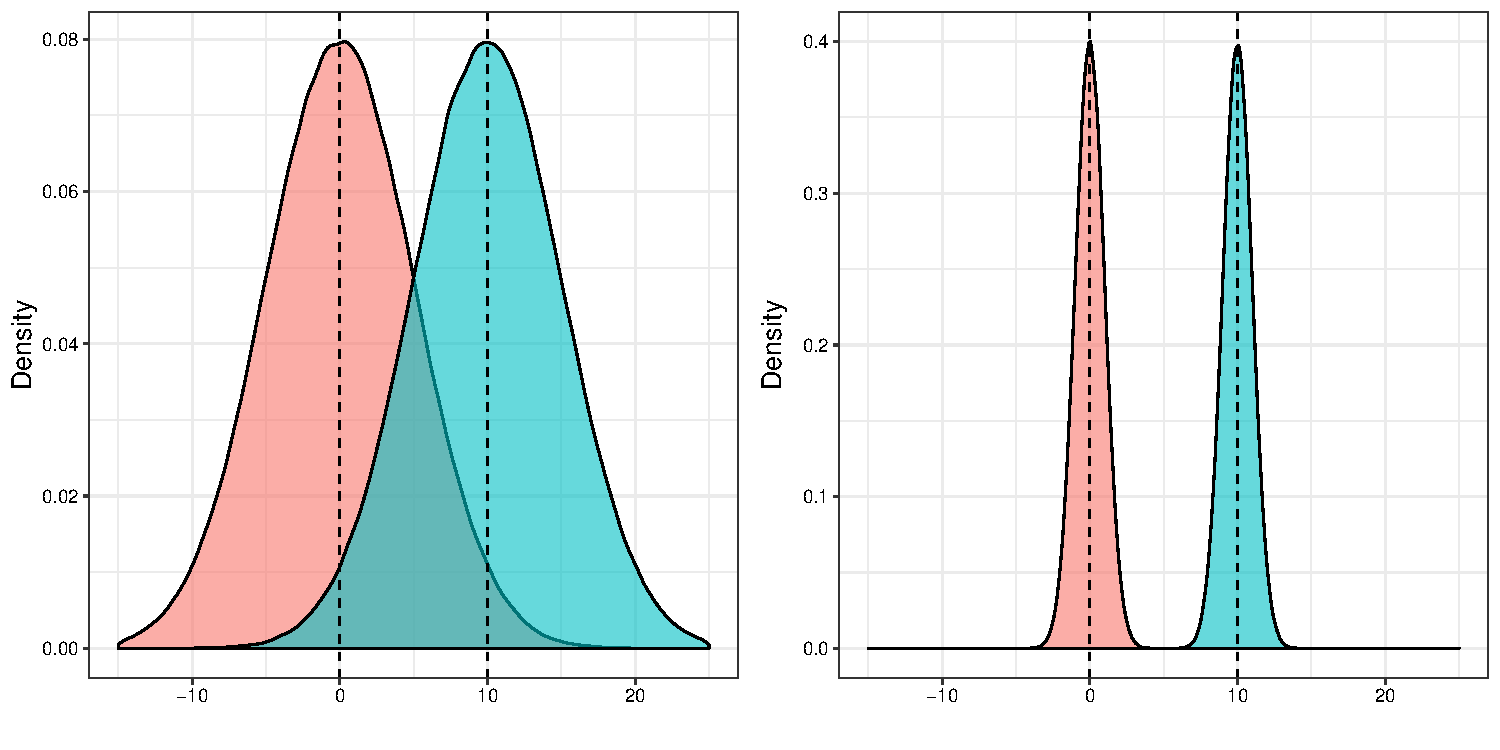
\includegraphics[width=0.75\textwidth]{rnorm.pdf}
		\caption{}
		\label{fig:XX}
	\end{center}
\end{figure}

Hence, rather than using the euclidean distance, it is more appropriate to use a KL divergence as a distance metric:
\[
	\nabla \Lagr(\bfX|\theta)_{KL} = \lim_{h\to0} \frac{1}{\|h\|}\argmax_{d \, s.t. KL[p_\theta||p_{\theta+d}]=\|h\|} \Lagr(\theta+d) - \Lagr(\theta)
\]
The direction of steepest ascent measured by the KL divergence is called the natural gradient.

To find the optimal $\hat{d}_{KL}$, one needs to solve the following optimisation problem:
\[
	\hat{d}_{KL} = \argmin_{d} \Lagr(\theta+d)
\]
with the constrain $KL[p_\theta||p_{\theta+d}]=c$, where $c$ is an arbitrary constant. Introducing Lagrange multipliers $\lambda$: \cite{??}:
\[
	\Lagr(\theta+d) + \lambda(KL[p_\theta||p_{\theta+d}] - c)
\]
Before taking its derivative, we can simplify the equation by approximating the  term $ \Lagr(\theta+d)$ with a First-order Taylor series and the term $KL[p_\theta||p_{\theta+d}]$ with a second-order Taylor series around $\theta+d$:
TO FINMISH
\[
KL[p_\theta||p_{\theta+d}]  \approx 
KL[p_\theta||p_{\theta}] + 
%d \d nabla_{\theta+d} KL[(\bfX|\theta)||(\bfX|\theta+d)] | _{\theta} +
%\frac{1}{2} d^T \d nabla^2_{\theta+d} KL[(\bfX|\theta)||(\bfX|\theta+d)] | _{\theta}d
\]
The first two terms vanish. The third term corresponds to the negative of the Hessian matrix with respect to $\theta+d$ (the Fisher Information Matrix $F$), evaluated at $\theta$. Hence, the term $KL[p_\theta||p_{\theta+d}]$ simplifies to $\frac{1}{2} d^T F d$

The equation to optimise becomes:
\[
\Lagr(\theta) + \nabla_{\theta} \Lagr(\theta)^T d + \frac{1}{2} \lambda d^T F d - \lambda c
\]

Finally, by taking the derivative of Equation X with respect to $d$, setting to zero and solving, we obtain the direction of the steepest natural gradient. It corresponds to the standard (euclidean) gradient pre-multiplied by the inverse of the Fisher Information Matrix:
\[
%	\frac{\partial \Lagr(\theta+d)}{\partial d} + \lambda\frac{\partial(KL[p_\theta||p_{\theta+d}]}{\partial d} = 0
\hat{d} \propto F^{-1} \nabla_{\theta} \Lagr(\theta)
\]


FINISH HERE. CHECK IF THE BOTTOM IS MEANINGFUL:::

Plugging this expression into [[EQUATION XX]], we find that the optimal $d$ is:
\[
\hat{d} = -\frac{1}{\lambda} F(\theta)^{-1} \nabla_{\theta} \Lagr(\theta)
\]
The constatn factor can be absorbed into the learning rate. The natural gradient is then defined
\[
\nabla \Lagr(\bfX|\theta)_{KL} = F(\theta)^{-1} \nabla_{\theta} \Lagr(\theta)
\]


% \cite{[[GITHUBPAGE]]} shows how, in a simple logistic regression problem, the use of natural gradients lead to improved convergence over standard gradient descent.